%!TEX root = ../Thesis.tex

\section{Design goals}
Virt-TAS is designed to fulfill the following goals:

\begin{enumerate}
    \item \textbf{Low latency and high throughput} % write about TAS
    Modern data-centers host distributed data-intensive applications, that require 
    low latency and high throughput. Workloads of these applications consist of short-lived 
    flows with stringent low latency requirements, as well as long-lived flows with 
    high throughput needs. VirtTAS should provide the latency and throughput needs 
    of these applications, and it should enable cloud providers to offer and maintain
    Service Level Agreements (SLAs). 
    
    \item \textbf{Compatibility} % write about openflow
    The networking interfaces should be unmodified so that applications residing on 
    the VMs could benefit from VirtTAS without any modification.
    Moreover, to make VirtTAS programmable through existing state-of-the-art network controllers,
    it should support OpenFlow API.

    \item \textbf{Coexistence with traditional Kernel networking}
    The new networking framework should be capable of working in conjunction with the 
    traditional virtual machine networking system. This allows tenants to execute certain
    workloads using the available kernel networking, while utilizing VirtTAS for
    performance-critical workloads.
    
    In order to ensure seamless coexistence, it is 
    necessary for VirtTAS to operate without adversely impacting the performance of 
    other applications that are running on the same machine. 

    \item \textbf{Resource efficiency}
    As VirtTAS shares fate with the hypervisor, resource conversation is highly critical. 
    VirtTAS should maximize resource efficiency to maintain precious resources for the 
    main goal of the hypervisor, running user workloads.

    \item \textbf{Scalability} % using a shared tcp fast-path
    Scalability becomes a challenging problem when different tenants with different network 
    topologies and networking demands reside on the same hypervisor. VirtTAS should keep up 
    with the increasing number of flows. It should also support an increasing number of flow 
    updates from a controller.
\end{enumerate}

    In order to advance the VirtTAS framework, several other goals have been identified for 
    future work. The pursuit of the following goals is expected to enhance the functionality 
    and effectiveness of our framework. 
    
\begin{itemize}
    \item \textbf{Mobility} % write about not being coupled to a physical network
    VMs could be migrated to different locations, thus VirtTAS should allow VMs to continue 
    communicating over the network, despite their migration. VirtTAS should decouple applications 
    from physical networking infrastructures at their location.
    \item \textbf{Isolation} 
    Applications residing on one VM must be prevented to access packets from other VMs. 
    They should not be able to violate other tenants' SLAs. Thus, VirtTAS should provide 
    the same isolation as the current architecture.

\end{itemize}

\section{Challenges}

\section{Design principles}
To achieve the aforementioned goals, we benefit from a set of design principles 
to provide network virtualization features in a shared TCP fastpath.

\section{Virt-TAS Architecture Overview}

Similar to TAS, Virt-TAS devides the network stack into three different components:
(\emph{i}) A fast-path running on hypervisor, (\emph{ii}) a slow-path that has components
both on the hypervisor and the VMs, and (\emph{iii}) an application library, which 
runs entirely on the VM side. 



\begin{figure}
    \centering
    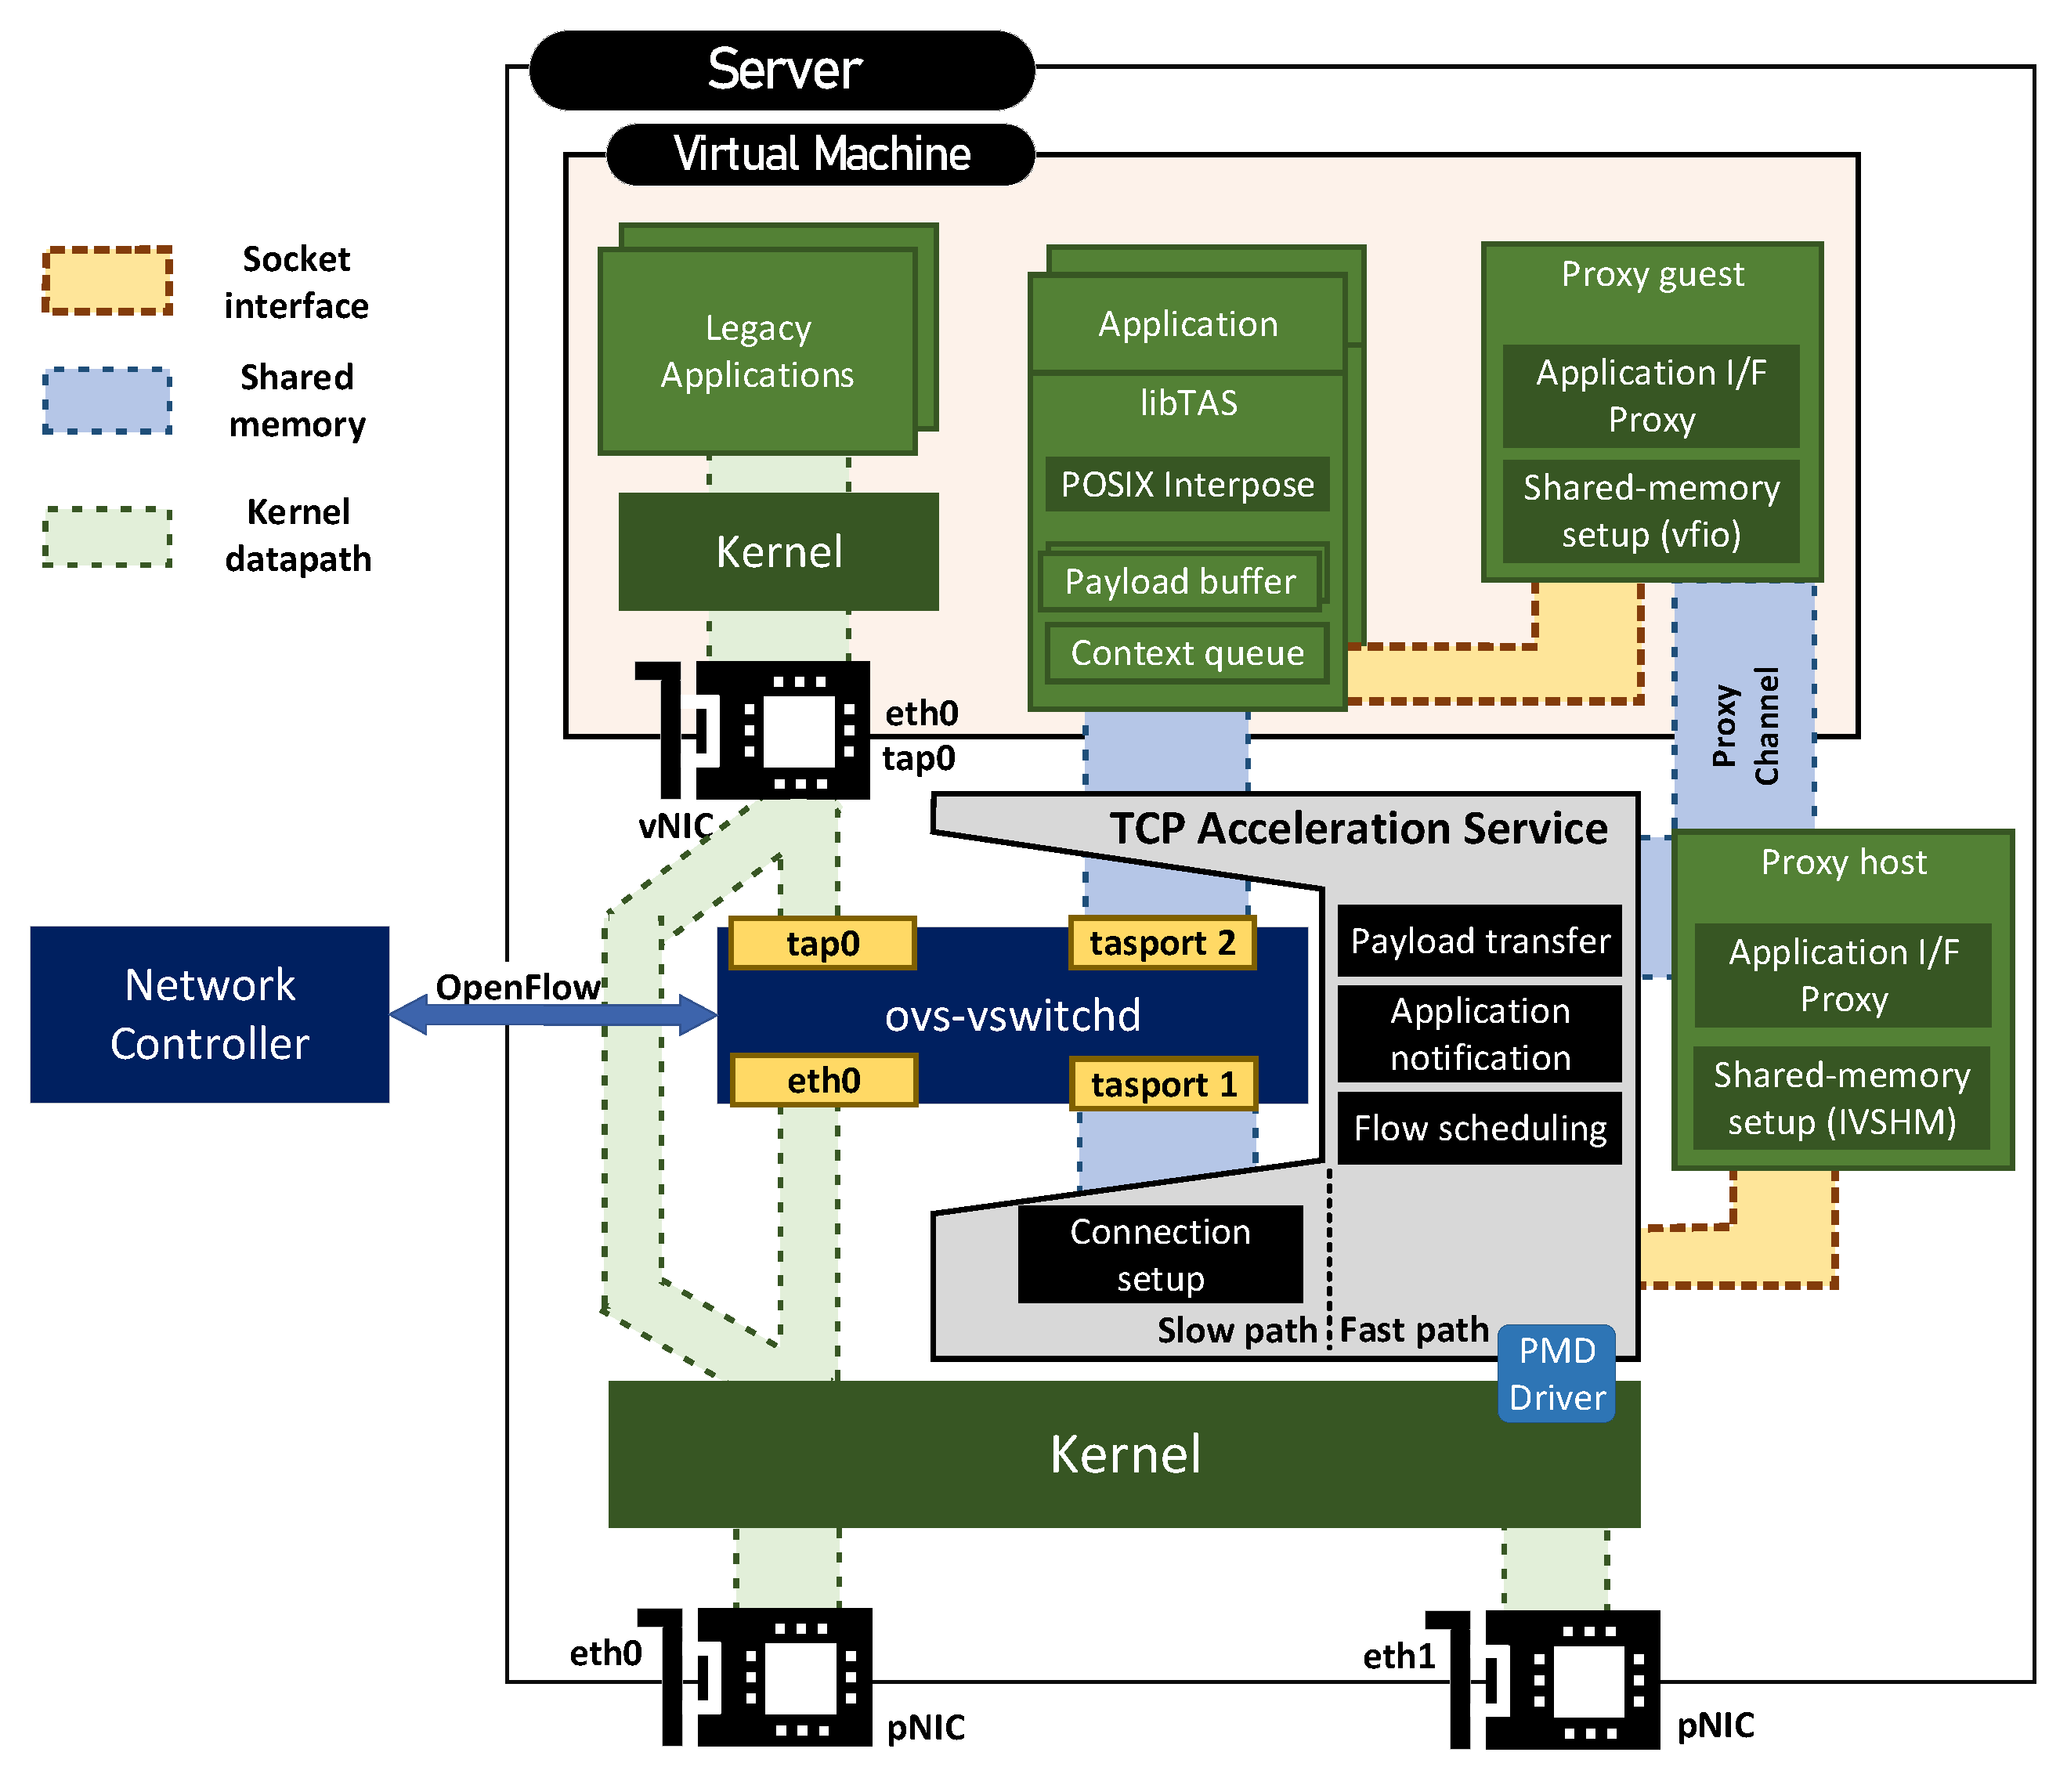
\includegraphics[scale=0.324]{../Figures/design.bigpicture.v2.pdf}
    \caption{Virt-TAS big picture}
    \label{fig:overhead.throughput}
\end{figure}


% a paragraph about the overview of ovs integration
Figure X depicts the overview architecture of Virt-TAS. The packets are first received 
by the fast-path component from a physical NIC or through shared memory from applications 
running on VMs. The fast-path either has received instruction from OVS on how to handle 
the received packet based on its flow or it has not. In the first scenario, the fast-path 
applies the action provided by OVS. The actions ranges from dropping the packet to forwarding 
it to specific application connected to Virt-TAS or to the physical NIC. In the second 
scenario, where fast-path has no information about the flow of the received packet,  the 
packet is delivered to OVS through lock-free shared memory. OVS can then decide how to treat 
packets. On the other side, the application interface has the responsibility to initialize the 
connection to Virt-TAS and implement POSIX network socket API for applications.

% a paragraph about the overview of sdn controller
By integrating OVS, we can control and program the forwarding dataplane through 
OpenFlow protocol. OpenFlow enables network operators to add, remove, update entries,
and to monitor statistics on flow tables. OVS takes OpenFlow tables from an SDN
controller, matches the received packets to these flow tables, and applies 
all actions needed to be taken. The outcome is then cached by the fast-path component
of Virt-TAS. This significantly simplifies the fast-path, as it allows the fast-path to 
be agnostic to OpenFlow specifics. One the other side, from the perspective of an OpenFlow 
controller,  processing packets in Virt-TAS is an invisible implementation detail. In its 
perspective, all packets are matched against multiple flow tables, and the corresponding 
actions are applied among entries that satisfy all conditions and have the highest priority.

% a paragraph about the proxy connection


% a paragraph about rediction of library calls 
A userspace library redirects the POSIX socket API transparently, so that applications 
remain unmodified. Through this library the sockets calls are transmitted to the 
hypervisor instead of being transfered to the VMs network stack. Furthermore, 
By rewriting applications to use low level API of libTAS higher performance can be achieved.

\section{Slow Path}
\subsection{Virtual switching}
\subsection{Proxy Host on hypervisor}

The Proxy Host is a service that operates on the hypervisor as an intermediary between virtual 
machines and the TAS. It uses the libtas library to connect to the running TAS instance on 
the hypervisor. The Proxy Host determines the number of supported groups from the TAS instance 
and sets up a UNIX socket for each group. The path of the created socket for the desired group 
is then used to launch virtual machines with fast-path support.
% [caption={qemu system x86_64 command with ivshmem-doorbell and socket to proxy host communication},captionpos=b^d%i]
\begin{lstlisting}[caption={QEMU system x86-64 command with ivshmem-doorbell and socket interface for connection to proxy host},captionpos=b]
qemu-system-x86_64 \
...
-chardev socket,path="PROXY_SOCKET_PATH",id="tas" \
-device ivshmem-doorbell,vectors=1,chardev="tas" \ 
...
\end{lstlisting}

runs a request to a server, it is sent to the proxy server first. The proxy server then makes a request to the server on behalf of the client, and returns the response back to the client.
\subsection{Proxy guest on VMs}
\subsection{Application Interface}

\section{Fast Path}
\subsection{Connection setup}
\subsection{OpenFlow action caching}

\section{Application library}